\input cinput.tex    \documentclass[12pt,fleqn,a4paper]{article}%
\usepackage{makeidx}
\makeindex
\usepackage{bm}
\usepackage{framed} % Easier way to use Framebox
\usepackage{pdfpages} % Import PDF in latex document
\usepackage{fancybox}
\usepackage{ulem} % for text strikethrough
\usepackage{tikz}
\usepackage{listings}
\usepackage{slashbox}
\usepackage{array}
\usepackage{enumitem}
\usepackage{amsmath, amssymb, amsthm}  % For mathematical symbols
\usepackage{rotating, booktabs}  % For table-rotating
\usepackage{longtable,booktabs}
\usepackage{wallpaper}  % For watermark
\usepackage{colortbl,color}
\usepackage{xcolor}
\usepackage{graphicx,psfrag}
\usepackage{tabularx,array}
\usepackage{booktabs}
\usepackage{multirow}
\usepackage{multicol}
\usepackage[subfigure]{tocloft}
\usepackage[tight]{subfigure}
\usepackage{float,booktabs,threeparttable}
\usepackage{caption}
\usepackage{menukeys}
\usepackage{pst-tree}
\usepackage{longtable}
\usepackage{appendix}
\usepackage{adjustbox}
\usepackage{pdfpages}

\def\se{{\rm se}}
%\newcommand{\red}{\color{red}}
\linespread{1.5}  % The linespread is 1.5.

% Numbered theorems, definitions, algorithm and lemmas ======================================================================
\newtheorem{thm}{Theorem}  % Define new theorem.
\newtheorem{alg}{Algorithm}[section]  % Define new algorithm.
\newtheorem{definition}{Definition}
% ===========================================================================================================================

% For writing pseudo code ======================================================================
\usepackage{algorithm}% http://ctan.org/pkg/algorithms
\usepackage{algpseudocode}% http://ctan.org/pkg/algorithmicx
% ===========================================================================================================================

\theoremstyle{definition}
\theoremstyle{plain}
\setcounter{secnumdepth}{5}


\renewcommand{\contentsname}{Table of Contents}
\renewcommand{\listfigurename}{List of Figures}
\renewcommand{\listtablename}{List of Tables}
\renewcommand{\figurename}{\footnotesize Figure}
\renewcommand{\tablename}{\footnotesize Table}
\newcommand{\loflabel}{Figure}
\newcommand{\lotlabel}{Table}
\setlength{\abovecaptionskip}{0pt}

%\renewcommand{\cftsecpresnum}{Chapter }

\renewcommand{\cftsecnumwidth}{7em}
%\renewcommand{\thesection}{{\ctxfbb Chapter}~~ \arabic{section}}
%\renewcommand{\thesubsection}{\arabic{section}.\arabic{subsection}}
%\renewcommand{\thesubsubsection}{\arabic{section}.\arabic{subsection}.\arabic{subsubsection}}
\renewcommand{\appendixpagename}{\LargeAppendix} % \ctxfb
\renewcommand{\arraystretch}{1.2}

\usepackage{appendix}

\def\oo{\nolinebreak[4]\hspace{.3em}\raise.7ex\hbox{{\MaQ\cH1}}\hspace{0.3em}}
\def\pp{\nolinebreak[4]\hspace{.3em}\raise.8ex\hbox{,}\hspace{0.3em}}
\def\dd{\nolinebreak[4]\hspace{.3em}\raise.8ex\hbox{{\MaQ\cH2}}\hspace{0.3em}}
\def\kk{\nolinebreak[4]\hspace{.3em}\raise.3ex\hbox{;}\hspace{0.3em}}
\def\mm{\nolinebreak[4]\hspace{.3em}\raise.3ex\hbox{:}\hspace{0.3em}}
\def\aa{\nolinebreak[4]\hspace{.3em}\raise.3ex\hbox{?}\hspace{0.3em}}

%%%%%%%%%%

%%%%%%%%%%
\usepackage[refpage]{nomencl}
\renewcommand{\nomname}{Notations}
\renewcommand*{\pagedeclaration}[1]{\unskip\dotfill\hyperpage{#1}}
\newcommand\independent{\protect\mathpalette{\protect\independenT}{\perp}}
\def\independenT#1#2{\mathrel{\rlap{$#1#2$}\mkern2mu{#1#2}}}
\makenomenclature
\usepackage{makeidx}
\makeindex
%%%%%%%%%%%%
%\let\clipbox\relax

%%%%%%%%%%%%
%\ctxfdef{\section}{\ctxfbb}
%\ctxfdef{\subsection}{\ctxfbb} %\ctxfr

\def\tb#1#2{\mathop{#1\vphantom{\sum}}\limits_{\displaystyle #2}}

\newtheorem{lma}{\textbf{Lemma}}

% ======================== Set length ========================
\setlength{\columnsep}{2.4cm}
\setlength\parindent{0pt}
\textheight=22cm
\textwidth=16.5cm
\hoffset=-1cm
% ============================================================


% =============================
% Equation numbering
\numberwithin{equation}{section}
% =============================

\begin{document}
\setcounter{section}{3}
\section{Classifications}
\subsection{\textbf{Logistic Regression}}
\subsubsection{\textbf{Logistic Model}}

logistic function:
\begin{gather}
p(x_{i}) = \frac{e^{\beta^{T}x_{i}}}{1+e^{\beta^{T}x_{i}}} = \frac{1}{1+e^{-\beta^{T}x_{i}}},~~ 0 \leq p(x_{i}) \leq 1, ~~ -\infty < x_{i} < \infty
\label{logistic-model}
\end{gather}

The logistic function will always produce an S-shaped curve.
\begin{figure}[H]
\centering
\psfrag{A}[c][l]{$X$}
\psfrag{B}[c][l]{$p(X)$}
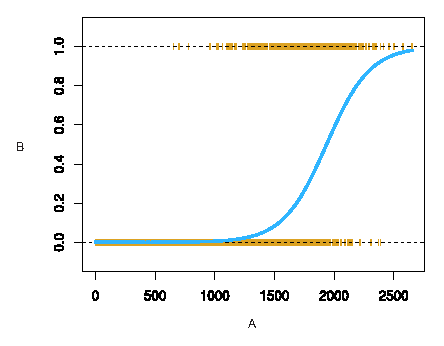
\includegraphics[scale=1]{images//4_2.eps}
\\~\\
\caption{}\label{figure-4.2}
\end{figure}

With a bit of manipulation, we will get a odds function:
\begin{gather}
\frac{p(x_{i})}{1-p(x_{i})} = e^{\beta^{T}x_{i}},~~ 0< \frac{p(x_{i})}{1-p(x_{i})} < \infty
\label{odds-function}
\end{gather}

The notation $p(x)$ can be interpreted as ${\rm Pr(Y=1|X=x)}$, which means the probability of $Y$ is True given $x$.
The equation \eqref{odds-function} imply the ratio of success compare to fail. For example, average nine of ten people go to school.
That means 9 times of people go to school compare to those who don't. So:
\begin{gather*}
p(x) = {\rm Pr(y=1|x)} = 9/10 \\
\frac{p(x)}{1-p(x)} = \frac{9/10}{1-9/10} = 9
\end{gather*}

By taking the logarithm of the odds function, we get
\begin{gather}
\log \bigg( \frac{p(x)}{1-p(x)} \bigg)= \beta^{T}x_{i}
\end{gather}

The left-hand side is called the log-odds or logit. We see that the logistic regression model has a logit that is linear in $X$.


\subsubsection{\textbf{Estimating the Regression Coefficients}}
To fit logistic model \eqref{logistic-model}, we use Maximum Likelihood to estimate the coefficients:
\begin{framed}
\begin{definition}[Likelihood Function]
~\\
$X_{1},X_{2},\dots,X_{n}$ {\MbQ\cH209}\z{\McQ\cH248}\z{\McQ\cH32}\z{\MbQ\cH154}\z{\MbQ\cH133}\z{\MaQ\cH215}\z{\MaQ\cH252}\z{\MbQ\cH209}$n${\MaQ\cH53}\z{\McQ\cH211}\z{\MbQ\cH156}\z{\MbQ\cH154}\z{\MbQ\cH133}, {\McQ\cH112}\z{\MbQ\cH209}$X_{1},X_{2},\dots,X_{n} \stackrel{i.i.d.}{\sim} f_{X_{i}}(x_{i};\theta)$, {\MaQ\cH236}\z{\McQ\cH50}\z{\MgQ\cH130}\z{\McQ\cH241}\z{\MaQ\cH161}\z{\MbQ\cH98} $\theta$ {\MaQ\cH53} likelihood function:
\begin{gather*}
L(\theta) = f_{X_{1},X_{2},\dots,X_{n}}(x_{1},x_{2},\dots,x_{n}) = \prod_{i=1}^{n}f_{X_{i}}(x_{i};\theta)
\end{gather*}
{\MaQ\cH170}\z{\McQ\cH106}\z{\MiQ\cH232}\z{\MbQ\cH209}\z{\MaQ\cH202}\z{\MaQ\cH46}\z{\MaQ\cH176}\z{\MbQ\cH237}\z{\MgQ\cH130}\z{\McQ\cH241}\z{\MaQ\cH161}\z{\MbQ\cH98}\z{\MdQ\cH77}$\theta${\MaQ\cH53}\z{\MaQ\cH45}, {\MfQ\cH130}\z{\MaQ\cH131}\z{\McQ\cH165}\z{\McQ\cH32}\z{\McQ\cH104}\z{\MgQ\cH191}\z{\MbQ\cH237}\z{\McQ\cH211}\z{\MbQ\cH156}\z{\MbQ\cH154}\z{\MbQ\cH133} ($X_{1},X_{2},\dots,X_{n}$) {\MaQ\cH53}\z{\MaQ\cH170}\z{\McQ\cH63}\z{\MbQ\cH52}
\end{definition}
\end{framed}

\textbf{\color{blue}{Maximum Likelihood Estimator, $\hat{\theta}_{\rm MLE}$}}:\\
{\MfQ\cH118}\z{\McQ\cH248}\z{\MaQ\cH95} $\theta$ {\MaQ\cH85}\z{\MbQ\cH41}\z{\MfQ\cH147}\z{\MaQ\cH131}\z{\McQ\cH165}\z{\McQ\cH32}\z{\McQ\cH211}\z{\MbQ\cH156}\z{\MbQ\cH154}\z{\MbQ\cH133} ($X_{1},X_{2},\dots,X_{n}$) {\MbQ\cH237}\z{\MaQ\cH170}\z{\McQ\cH63}\z{\MbQ\cH52}\z{\MbQ\cH209}\z{\MbQ\cH124}\z{\MaQ\cH215}, {\MaQ\cH63}\z{\MdQ\cH185}, {\MfQ\cH118}\z{\McQ\cH248}\z{\MaQ\cH95} $\theta$ {\MaQ\cH85}\z{\MbQ\cH41}\z{\MbQ\cH150}\z{\MaQ\cH78}\z{\MdQ\cH131}\z{\MbQ\cH98} $L(\theta)$ {\MbQ\cH209}\z{\MbQ\cH124}\z{\MaQ\cH215}:
\begin{gather*}
\text{arg}\,\max\limits_{\theta}\,L(\theta), \text{{\MbQ\cH176}\z{\McQ\cH106}}\,\hat{\theta}_{\rm MLE}
\end{gather*}

Unlike linear regression, we can no longer write down the MLE in closed form.
Instead, we need to use an optimization algorithm to compute it.
For this, we need to derive the gradient and Hessian. The likelihood function of logistic model:

\begin{gather}
L(\beta) = \prod_{i=1}^{n} p(x_{i};\beta)^{y_{i}} (1-p(x_{i};\beta))^{1-y_{i}},~\text{where~} R_{y_{i}}=\{0,1\}
\end{gather}

The log-likelihood of logistic model:
\begin{align*}
\ell(\beta)& = \sum\limits_{i=1}^{n} y_{i} \log p(x_{i};\beta)+(1-y_{i})\log (1-p(x_{i};\beta)) \\
		   & = \sum\limits_{i=1}^{n} y_{i} \log p(x_{i};\beta) + \log (1-p(x_{i};\beta)) - y_{i} \log (1-p(x_{i};\beta))\\
		   & = \sum\limits_{i=1}^{n} y_{i} \log \frac{p(x_{i};\beta)}{1-p(x_{i};\beta)} + \log (1-p(x_{i};\beta))  \\
		   & = \sum\limits_{i=1}^{n} y_{i}\beta^{T}x_{i}+ \log (\frac{1}{1+e^{\beta^{T}x_{i}}}) \\
 		   & = \sum\limits_{i=1}^{n} \{y_{i}\beta^{T}x_{i}-\log (1+e^{\beta^{T}x_{i}})\}
\end{align*}

First order partial differential of the log-likelihood function (gradient descent):
\begin{align*}
\frac{\partial \ell(\beta)}{\partial \beta} & = \sum\limits_{i=1}^{n} x_{i}(y_{i} - \frac{e^{\beta^{T}x_{i}}}{1+e^{\beta^{T}x_{i}}}) \\
 & = \sum\limits_{i=1}^{n} x_{i}(y_{i} - p(x_{i};\beta))
\end{align*}

Second order partial differential of the log-likelihood function (the s.o.c can transfer to a Hessian matrix):
\begin{align*}
\frac{\partial^{2} \ell(\beta)}{\partial \beta \partial \beta^{T}}
 & = \sum\limits_{i=1}^{n} x_{i}(-x_{i} \cdot \frac{e^{-\beta^{T} x_{i}}}{1+e^{-\beta^{T} x_{i}}} \cdot \frac{1}{1+e^{-\beta^{T} x_{i}}}) \\
 & = -\sum\limits_{i=1}^{n} x_{i}x_{i}^{T} p(x_{i};\beta) (1-p(x_{i};\beta))
\end{align*}

Starting with $\beta^{old}$, a single Newton update is
\begin{gather*}
\beta^{new} = \beta^{old} - \bigg(\frac{\partial^{2} \ell(\beta)}{\partial \beta \partial \beta^{T}}\bigg)^{-1} \frac{\partial \ell(\beta)}{\partial \beta}
\end{gather*}

Now we will try to simplify by vectorizing the model. Let $\mathbf{y}$ denote the vector of $y_{i}$,
$\mathbf{X}$ the $N \times (p+1)$ matrix of $x_{i}$ ($p$ predictors with one intercept),
$\mathbf{p}$ the vector of fitted probabilities with $i$th element $p(x_{i};\boldsymbol{\beta}^{\text{old}})$ and
$\mathbf{W}$ a $N \times N$ diagonal matrix of weights with $i$th diagonal element $p(x_{i};\boldsymbol{\beta}^{\text{old}})(1-p(x_{i};\boldsymbol{\beta}^{\text{old}}))$.
The structure of the notation and the model: ~\\~\\

$
\mathbf{y}_{N \times 1} = \begin{pmatrix}
  y_{1}  \\
  y_{2}  \\
  \vdots  \\
  y_{N}
 \end{pmatrix}
$,
$
\mathbf{X}_{N \times (p+1)} = \begin{pmatrix}
  1 & x_{11} & x_{12} & \cdots & x_{1p} \\
  1 & x_{21} & x_{22} & \cdots & x_{2p} \\
  \vdots & \vdots & \vdots & \ddots & \vdots  \\
  1 & x_{N1} & x_{N2} & \cdots & x_{Np}
 \end{pmatrix}
$, ~\\

$
\mathbf{p}_{N \times 1} = \begin{pmatrix}
  p(x_{1};\boldsymbol{\beta}^{\text{old}})  \\
  p(x_{2};\boldsymbol{\beta}^{\text{old}})  \\
  \vdots  \\
  p(x_{N};\boldsymbol{\beta}^{\text{old}})
 \end{pmatrix}
$,
$
\boldsymbol{\beta}^{\text{old}}_{(p+1) \times 1} = \begin{pmatrix}
  \beta_{0}  \\
  \beta_{1}  \\
  \beta_{2}  \\
  \vdots  \\
  \beta_{p}
 \end{pmatrix}
$,

\begin{gather*}
\footnotesize
\mathbf{W}_{N \times N} = \begin{pmatrix}
  p(x_{1};\boldsymbol{\beta}^{\text{old}})(1-p(x_{1};\boldsymbol{\beta}^{\text{old}})) & 0 & \cdots & 0 \\
  0 & p(x_{2};\boldsymbol{\beta}^{\text{old}})(1-p(x_{2};\boldsymbol{\beta}^{\text{old}})) & \cdots & 0 \\
  \vdots & \vdots & \ddots & \vdots  \\
  0 & 0 & \cdots & p(x_{N};\boldsymbol{\beta}^{\text{old}})(1-p(x_{N};\boldsymbol{\beta}^{\text{old}}))
 \end{pmatrix}
\end{gather*}

\begin{align*}
\frac{\partial \ell(\beta)}{\partial \beta} & = \mathbf{X}^{T}(\mathbf{y}-\mathbf{p}) \\
\frac{\partial^{2} \ell(\beta)}{\partial \beta \partial \beta^{T}}  & = -\mathbf{X}^{T} \mathbf{W} \mathbf{X} \\
\boldsymbol{\beta}^{\text{new}} &= \boldsymbol{\beta}^{\text{old}} + \big( \mathbf{X}^{T} \mathbf{W} \mathbf{X} \big)^{-1} \mathbf{X}^{T}(\mathbf{y}-\mathbf{p}) \\
 & = \big( \mathbf{X}^{T} \mathbf{W} \mathbf{X} \big)^{-1} \mathbf{X}^{T} \mathbf{W} \big( \mathbf{X} \boldsymbol{\beta}^{\text{old}} +  \mathbf{W}^{-1}(\mathbf{y}-\mathbf{p})\big) \\
 & = \big( \mathbf{X}^{T} \mathbf{W} \mathbf{X} \big)^{-1} \mathbf{X}^{T} \mathbf{W} \mathbf{z}
\end{align*}

Response of weighted least squares step, sometimes known as adjusted response:
\begin{gather}
\mathbf{z} = \mathbf{X} \boldsymbol{\beta}^{\text{old}} +  \mathbf{W}^{-1}(\mathbf{y}-\mathbf{p})
\end{gather}

The equations above solved repeatedly, since at each iteration $\mathbf{p}$ changes, and hence so does $\mathbf{W}$ and $\mathbf{z}$.
This algorithm is referred to as iteratively reweighed least squares (IRLS).

\begin{algorithm}[H]
\caption{Iteratively reweighted least squares (IRLS)}\label{euclid}
\begin{algorithmic}[1]
\State $\boldsymbol{\beta}^{\text{new}} =  \begin{pmatrix}  1 \\ \boldsymbol{\mathbf{\beta}}_{p}  \end{pmatrix} ;$
\Repeat
\State $\mathbf{p} = p(\mathbf{X};\boldsymbol{\beta}^{\text{new}})$
\State $\mathbf{W}_{N \times N} = \text{diag}(\mathbf{p} (1-\mathbf{p}))$
\State $\mathbf{z} = \mathbf{X}\boldsymbol{\beta}^{\text{new}}+ \mathbf{w}^{-1}(\mathbf{y}-\mathbf{p})$
\State $\boldsymbol{\beta}^{\text{new}} = (\mathbf{X}^{T} \mathbf{W} \mathbf{X})^{-1} \mathbf{X}^{T} \mathbf{W} \mathbf{z} $
\Until{calculate loss function to check converged;}
\end{algorithmic}
\end{algorithm}

\subsubsection{Discussion}
\begin{enumerate}
\item How to calculate the fitness of logistic model?
\item How to check the estimated coefficients is significant or not?
\item How to perform the hypothesis testing for logistic regression? 
\item What is the assumptions of logistic regression model?
\end{enumerate}

\subsection{\textbf{Linear Discriminant Analysis (LDA)}}

Difference between Linear Discriminant Analysis and Logistic Analysis:
\begin{itemize}
\item when the classes are well-separated, the parameter estimates for the logistic regression model are surprisingly unstable. LDA does not suffer from this problem
\item If $n$ is small and the distribution of the predictors $X$ is approximately normal in each of the classes, LDA is more stable than logistic regression
\item LDA is preferable when we have more than two response classes.
\item Logistic regression can take both qualitative and quantitative as predictor variables. However LDA can only take quantitative predictor variables, due to the assumption of multivariate Gaussian Distribution.
\item LDA assumes that the classes have a common covariance matrix
(Continuous random variable $X$)
\end{itemize}

\subsubsection{\textbf{Bayes Theorem for Classification}}
Classify an observation into one of $K$ classes, where $K \geq 2$.

Notations: 
\begin{itemize}
\item $Y$: The qualitative response variable with $K$ different categories, $R_{Y} = {1,\dots,K}$
\item $\pi_{k}$: The prior probability that a randomly chosen observation comes from the $k$th class
\item $f_{k}(X)$: the density function of $X$ for an observation comes form the $k$th class
\end{itemize}

\begin{framed}
Note:
\begin{gather*}
\hat{\pi}_{k} = n_{k}/n = \hat{Pr}(Y=k) \\
f_{k}(X) = Pr(X=x|Y=k)
\end{gather*}
\end{framed}
From the law of total probability, the above notations can be stated as below:
\begin{gather}
Pr(Y=k|X=x) = \frac{\pi_{k}f_{k}(x)}{\sum\limits_{\ell=1}^{K}\pi_{\ell}f_{\ell}(x)}
\label{lda}
\end{gather}
The abbreviation for $Pr(Y=k|X=x)$ will be denoted as $p_{k}(X)$ which is the posterior probability that an observation $X=x$ belongs to the $k$th class.
In the following section, we have to make assumptions and approximates $f_{k}(X)$ to build a classifier that approximates the Bayes classifier.

\begin{framed}
\begin{definition}[The law of total probability]
~\\
{\McQ\cH113} $A_{1},A_{2},\dots,A_{n}$ {\MbQ\cH209}\z{\MbQ\cH154}\z{\MbQ\cH133}\z{\McQ\cH11}\z{\McQ\cH200}$S${\MaQ\cH50}\z{\MaQ\cH53}\z{\McQ\cH248}\z{\McQ\cH32}\z{\MaQ\cH125}\z{\MdQ\cH146}, {\MaQ\cH134}\z{\MaQ\cH250}\z{\MbQ\cH107}\z{\MbQ\cH154}\z{\MbQ\cH133}\z{\McQ\cH11}\z{\McQ\cH200}$S${\MaQ\cH53}\z{\MaQ\cH76}\z{\MbQ\cH60}\z{\MaQ\cH57}\z{\MaQ\cH75}$B${\McQ\cH55}\z{\McQ\cH107},
\begin{gather*}
P(B) = \sum\limits_{i=1}^{n}P(B|A_{i})P(A_{i})
\end{gather*}

\end{definition}
\end{framed}

\subsubsection{\textbf{Linear Discriminant Analysis for p=1}}
In the assumption of the Linear Discriminant Analysis, we assume the independent variable $X$ follow Gaussian distribution.
So the $f_{k}(x)$ takes the form
\begin{gather}
f_{k}(x) = \frac{1}{\sqrt{2\pi}\sigma_{k}}e^{-\frac{1}{2\sigma_{k}^{2}}(x-\mu_{k})^{2}}
\end{gather}
LDA also assume homoscedasticity for $\sigma_{1}^{2}=\sigma_{2}^{2}=\dots=\sigma_{K}^{2}$, so the simplify version of $f_{k}(x)$
\begin{gather}
f_{k}(x) = \frac{1}{\sqrt{2\pi}\sigma}e^{-\frac{1}{2\sigma^{2}}(x-\mu_{k})^{2}}
\label{lda_normal}
\end{gather}

By plugging \eqref{lda_normal} into \eqref{lda}, we get
\begin{gather}
p_{k}(x) = \frac{\pi_{k} \frac{1}{\sqrt{2\pi}\sigma}e^{-\frac{1}{2\sigma^{2}}(x-\mu_{k})^{2}}}{\sum\limits_{\ell=1}^{K}\pi_{\ell} \frac{1}{\sqrt{2\pi}\sigma}e^{-\frac{1}{2\sigma^{2}}(x-\mu_{\ell})^{2}}}
\end{gather}

In order to estimate the parameters from \eqref{lda_normal}, we apply MAP,
\begin{align}
\begin{split}
\hat{p}_{k} &= \arg\max_{k} P(Y=k|X=x) \\
		    &= \arg\max_{k} \pi_{k}f_{k}(x)\\
\end{split}
\label{MAP}
\end{align}

The objective of LDA is to find a $k$ that maximizes posterior probability($\hat{p}_{k}$) among all $K$th posterior probabilities. 
From the above model, in order to meet this objective, we will try to find a $k$ which will maximize the conditional probability ($\pi_{k}f_{k}(x)$).
Since, the maximum of $\pi_{k}f_{k}(x)$, imply the largest probability among all $K$th posterior probabilities.
In order to simplify \eqref{MAP}, we take the log of \eqref{MAP}

\begin{align}
\begin{split}
\arg\max_{k}  \delta_{k}(x) &= \arg\max_{k} \bigg( \log \pi_{k} + x \frac{\mu_{k}}{\sigma^{2}}-\frac{\mu_{k}^{2}}{2\sigma^{2}}+ \underline{\log \frac{1}{\sqrt{2\pi}\sigma}-\frac{x^{2}}{2\sigma^{2}}} \bigg)\\
 						    &= \arg\max_{k} \bigg( \log \pi_{k} + x \frac{\mu_{k}}{\sigma^{2}}-\frac{\mu_{k}^{2}}{2\sigma^{2}}+ \text{\sout{constant}} \bigg)
\end{split}
\end{align}

In practice we don't know the parameters of the Gaussian distributions(unknown $\mu_{k}, \sigma^{2}$), and will need to estimate them using our training data:

\begin{itemize}
\item $\hat{\pi}_{k} = n_{k}/n$
\item $\hat{\mu}_{k}=\sum\limits_{i:y_{i}=k}x_{i}/n_{k}$
\item $\hat{\sigma}^{2} = \sum\limits_{k=1}^{K}\sum\limits_{i:y_{i}=k}(x_{i}-\hat{\mu}_{k})^{2}/(n-k)$
\end{itemize}

The discriminant function,
\begin{gather}
\arg\max_{k}  \hat{\delta}_{k}(x) = \arg\max_{k} \bigg( \big( \log \hat{\pi_{k}} -\frac{\hat{\mu_{k}}^{2}}{2 \hat{\sigma^{2}}} \big) + x \frac{\hat{\mu}_{k}}{\hat{\sigma}^{2}} \bigg)
\label{discriminantfunction}
\end{gather}
The reason linear in the name of LDA, is because the discriminant functions are linear functions of $x$

\subsubsection{\textbf{Linear Discriminant Analysis for $p > 1$}}
Assume that $X = \big( X_{1}~~X_{1}~~\dots~~X_{p} \big)$ drown from a multivariate Gaussian distribution, with a class-specific mean vector and a common covariance matrix.
To indicate that a $p$-dimensional random variable $X$ has a multivariate Gaussian Distribution, we write $X \sim N(\mu,\sum)$


\subsubsection{Discussion}
\begin{enumerate}
\item What is the definition of Maximum a posteriori estimation(MAP)?
\item What is the Bayes decision boundary when $K=2$ ? What is the Bayes decision boundary when $K>2$ ?
\item What is Fisher linear discriminant function ?
\end{enumerate}

\section*{Reference}
\noindent
\begin{description}\itemsep=-2pt
\item {\MbQ\cH34}\z{\MiQ\cH16} (2012), {\MaQ\cH7}{\MbQ\cH84}\z{\MhQ\cH229}\z{\MeQ\cH78}\z{\McQ\cH228}\z{\MaQ\cH231}\z{\McQ\cH36}\z{\McQ\cH108}{\MaQ\cH8}, {\McQ\cH251}\z{\MhQ\cH23}, {\MkQ\cH49}\z{\MiQ\cH95}\z{\MaQ\cH199}\z{\MbQ\cH122}
\item Friedman, J., Hastie, T., \& Tibshirani, R. (2001). {\it{The elements of statistical learning}} (Vol. 1). Springer, Berlin: Springer series in statistics.
\item James, G., Witten, D., Hastie, T., \& Tibshirani, R. (2013). {\it{An introduction to statistical learning}} (Vol. 6). New York: springer.
\item Wasserman, L. (2013). {\it{All of statistics: a concise course in statistical inference}}. Springer Science \& Business Media.
\end{description}

\end{document}
